% ============================================================================
% Guided MATLAB coding tutorial: a universal-variables Lambert solver,
% built from Stumpff functions up through the full multi-revolution case.
% Checkpoints verified against pyKep (Izzo) -- the exact routine
% pumpkyn.pykep.lambert2Body wraps -- and against Vallado Example 7-5.
% All checkpoint numbers produced headlessly (R2025b) on 2026-07-06 via
% verify_lambert_checkpoints.m in this folder.
% ============================================================================
\documentclass[11pt,letterpaper]{article}
\usepackage[margin=1in]{geometry}
\usepackage{amsmath,amssymb,bm}
\usepackage{booktabs}
\usepackage{enumitem}
\usepackage{xcolor}
\usepackage{graphicx}
\usepackage[colorlinks=true,linkcolor=blue!70!black,urlcolor=blue!70!black]{hyperref}
\usepackage{fancyhdr}
\usepackage{titlesec}
\usepackage{mathtools}
\usepackage{tcolorbox}

\pagestyle{fancy}
\fancyhf{}
\rhead{Lambert Solver --- Guided Exercises}
\lhead{}
\rfoot{Page \thepage}
\setlength{\headheight}{14pt}

\setlength{\parskip}{5pt}
\setlength{\parindent}{0pt}

\titlespacing*{\section}{0pt}{14pt}{6pt}
\titlespacing*{\subsection}{0pt}{10pt}{4pt}

% --- convenience macros ---
\newcommand{\R}{\mathbb{R}}
\newcommand{\T}{^{\mathsf{T}}}
\newcommand{\half}{\tfrac12}
\newcommand{\rvec}{\mathbf{r}}
\newcommand{\dth}{\Delta\theta}

% --- Exercise: what the learner writes (blue) ---
\newtcolorbox{exercise}[1]{
  colback=blue!5!white, colframe=blue!50!black, fonttitle=\bfseries,
  title={Exercise: #1}, sharp corners, boxrule=0.8pt,
  left=6pt, right=6pt, top=4pt, bottom=4pt}

% --- Hint: partial code / gotcha nudge (yellow) ---
\newtcolorbox{hint}{
  colback=yellow!5!white, colframe=yellow!60!black, fonttitle=\bfseries,
  title={Hint}, sharp corners, boxrule=0.5pt,
  left=6pt, right=6pt, top=4pt, bottom=4pt}

% --- Checkpoint: runnable test with VERIFIED expected output (green) ---
\newtcolorbox{checkpoint}[1]{
  colback=green!5!white, colframe=green!50!black, fonttitle=\bfseries,
  title={Checkpoint: #1}, sharp corners, boxrule=0.8pt,
  left=6pt, right=6pt, top=4pt, bottom=4pt}

\title{\textbf{Building a Universal-Variables Lambert Solver}\\[8pt]
\large Guided Coding Exercises\\[4pt]
\normalsize From Stumpff functions to the full multi-revolution solution set,\\
verified against pyKep (the engine inside \texttt{pumpkyn.pykep.lambert2Body})}
\author{}
\date{July 2026}

\begin{document}
\maketitle
\tableofcontents
\newpage

% ==========================================================================
\section{Introduction}

You will build, from scratch in base MATLAB, a complete \textbf{Lambert
solver} in the universal-variables formulation: given two position vectors
and a time of flight, recover the connecting two-body orbit --- elliptic,
parabolic, or hyperbolic, prograde or retrograde --- and, in the finale,
\emph{every} solution including the multi-revolution branches.

The payoff is a three-way agreement your own code participates in: your
solver, \textbf{pyKep} (Izzo's solver --- the exact C++ routine that
\texttt{pumpkyn.pykep.lambert2Body} wraps), and \textbf{Vallado's textbook
Example 7-5} all produce the same velocities --- your build matches pyKep to
$10^{-15}$--$10^{-14}$ on single-rev cases and to $\sim$$10^{-13}$ across all
13 solutions of the multi-rev finale. The closing picture
(Figure~\ref{fig:expected}) is worth the build by itself: a U-shaped
time-of-flight curve crossed 13 times by one horizontal line, and the 13
corresponding orbits all threading the same two points.

\subsection{Prerequisites}

\begin{itemize}[leftmargin=*,nosep]
\item The orbit-transfer tutorial's astrodynamics primer
  (\texttt{optimal\_control/orbit\_transfer/}, \S1.2): canonical units,
  circular speed, the force law. This tutorial reuses those conventions
  ($\mu = 1$, positions in DU, times in TU).
\item Comfort with root-finding (bisection, brackets) and basic orbital
  mechanics vocabulary at the level of that primer. No prior exposure to
  Lambert theory is assumed --- \S\ref{sec:theory} is self-contained.
\item MATLAB R2025b. Base MATLAB only --- no toolboxes needed (the
  round-trip checks use \texttt{ode89}, which ships with core MATLAB).
\end{itemize}

\subsection{Lambert's problem in one page}\label{sec:theory}

\textbf{The problem.} Given $\rvec_1$, $\rvec_2$, and a flight time
$\Delta t$, find the coasting orbit connecting them: equivalently the
velocity $\mathbf{v}_1$ at $\rvec_1$ that arrives at $\rvec_2$ exactly
$\Delta t$ later under $\ddot\rvec = -\mu\rvec/r^3$. It is the two-body
\emph{boundary-value} problem (propagation is the initial-value problem),
and it is the workhorse of transfer design and initial orbit determination.

\textbf{What's fixed and what's free.} The transfer plane is dictated ---
it must contain $\rvec_1$, $\rvec_2$, and the \emph{focus} (the central
body's location, which every conic orbit keeps at one of its foci) --- so
the choice collapses to: which way around (\emph{prograde} =
counter-clockwise as seen from $+z$, \emph{retrograde} = clockwise, giving
transfer angle $\dth$ or $2\pi - \dth$), and how many complete revolutions
$N$ before arrival. For fixed sense and $N$, Lambert's theorem says the
flight time depends on one remaining parameter --- so the solver is
one-dimensional root-finding.

\textbf{The universal variable.} We use $z$, related to the change in
\emph{eccentric anomaly} $\Delta E$ --- the angle that parametrizes
progress around an ellipse (Kepler's equation lives in it); $\Delta H$ is
its hyperbolic analog --- by $z = \Delta E^2$ (elliptic),
$z = -\Delta H^2$ (hyperbolic), $z = 0$ (parabolic). One variable sweeps
continuously across all three conic regimes --- that is the entire point
of the formulation:
\begin{gather*}
  z < 0 \;\text{hyperbolic},\qquad z = 0 \;\text{parabolic},\qquad
  0 < z < (2\pi)^2 \;\text{elliptic (0-rev)},\\
  z \in \bigl((2\pi N)^2, (2\pi(N{+}1))^2\bigr)\;\text{elliptic, $N$ complete revolutions}.
\end{gather*}

\textbf{Solution count.} On the 0-rev domain the flight time $t(z)$
crosses any $\Delta t > 0$ exactly once. On each $N$-rev band $t(z)$ is
U-shaped with an interior minimum $t_{\min}(N)$, increasing in $N$: two
solutions if $\Delta t > t_{\min}(N)$, one double root in the
measure-zero tangent case $\Delta t = t_{\min}(N)$, none below. Total:
$2N_{\max} + 1$ --- the convention pyKep uses, and the count your finale
reproduces (13, for the tutorial instance).

\subsection{What ``verified against pumpkyn'' means here}

pumpkyn's two-body Lambert is \texttt{pumpkyn.pykep.lambert2Body}, a MEX
wrapper around Izzo's pyKep solver. The shipped MEX binaries are Linux and
Windows only, and as of 2026-07-06 the auto-compile path fails on this
Mac (a machine-wide C++ MEX toolchain fault --- MATLAB's own shipped C++
example fails identically). The checkpoint numbers were therefore produced
by compiling the \emph{same bundled source}
(\texttt{lambert\_original.cpp}) as a standalone command-line harness with
\texttt{clang++} --- byte-identical algorithmically to what
\texttt{lambert2Body} returns on the other platforms, and cross-anchored
against Vallado's published example. Provenance script:
\texttt{verify\_lambert\_checkpoints.m}.

\subsection{What you will build}

\begin{center}
\begin{tabular}{lp{9.4cm}}
\toprule
File & Purpose \\
\midrule
\texttt{stumpff.m}             & Stumpff functions $C(z)$, $S(z)$ with series near $z=0$ \\
\texttt{lambert\_tof.m}        & Flight time $t(z)$ for fixed endpoint geometry \\
\texttt{lambert\_uv.m}         & Single-rev solver: bracket, bisect, $f$-and-$g$ velocities \\
\texttt{lambert\_uv\_multirev.m} & All $2N_{\max}{+}1$ solutions: band minima + branch roots \\
\texttt{run\_lambert\_demo.m}  & The 13-solution finale, printed and plotted \\
\bottomrule
\end{tabular}
\end{center}

\subsection{Workspace split}

Build in \texttt{lambert/mytry/}; the parent folder holds the reference
solutions, consulted only after attempting each exercise (same protocol as
the orbit-transfer tutorial).

\subsection{Notation recap}

$\rvec_1, \rvec_2 \in \R^3$ endpoint positions, $r_1 = \|\rvec_1\|$ etc.;
$\dth$ transfer angle; $\mu$ gravitational parameter (canonical: 1);
$C(z), S(z)$ Stumpff functions; $y(z)$ the universal-variables intermediate;
$\chi = \sqrt{y/C}$ the universal anomaly; sense flag \texttt{dir} $= +1$
prograde / $-1$ retrograde (matching \texttt{lambert2Body}). The tutorial
instance used by most checkpoints:
\[
  \mu = 1,\qquad \rvec_1 = [1;0;0],\qquad \rvec_2 = [0;1.2;0],\qquad
  \text{prograde} \;(\dth = 90^\circ).
\]

% ==========================================================================
\section{Phase A: the Stumpff functions}

The universal formulation buys its all-conics generality with two special
functions, the cosine- and sine-like pair
\[
  C(z) = \frac{1 - \cos\sqrt z}{z},\qquad
  S(z) = \frac{\sqrt z - \sin\sqrt z}{z^{3/2}} \qquad (z > 0),
\]
and, for $z < 0$ (writing $w = -z > 0$),
\[
  C(z) = \frac{\cosh\sqrt w - 1}{w},\qquad
  S(z) = \frac{\sinh\sqrt w - \sqrt w}{w^{3/2}}.
\]
(Write these out rather than pattern-matching ``$\cos\to\cosh$'' --- the
naive substitution flips the sign of $S$.) They are smooth through $z = 0$
--- but their closed forms are $0/0$ there, which is where implementations
go wrong.

\begin{exercise}{\texttt{stumpff.m}}
Create
\begin{verbatim}
function [C, S] = stumpff(z)
\end{verbatim}
returning both functions, \textbf{elementwise for array} $z$ (Phase~B will
plot them over thousands of points). Three regimes: closed forms for
$z \ge 10^{-4}$ and $z \le -10^{-4}$, and a truncated Taylor series in
between. Derive the series yourself from
$\cos\sqrt z = 1 - z/2 + z^2/24 - \dots$: you should get
\[
  C(z) = \tfrac12 - \tfrac{z}{24} + \tfrac{z^2}{720} - \tfrac{z^3}{40320},
  \qquad
  S(z) = \tfrac16 - \tfrac{z}{120} + \tfrac{z^2}{5040} - \tfrac{z^3}{362880}.
\]
\end{exercise}

\begin{hint}
Use logical-index masks (\texttt{small = abs(z) < 1e-4}, etc.) rather than
a loop, and note the hyperbolic branch is cleanest computed with
$w = -z > 0$: \texttt{C = (cosh(sqrt(w)) - 1)./w}. With four series terms
the switchover error at $|z| = 10^{-4}$ is far below double precision ---
the checkpoint measures it.
\end{hint}

\begin{checkpoint}{A --- Stumpff values and the seam}
\begin{verbatim}
[C0,S0] = stumpff(0)                      % 0.5 and 1/6
[Cp,Sp] = stumpff(pi^2);  [Cp - 2/pi^2,  Sp - 1/pi^2]
[Cn,Sn] = stumpff(-4);
[Cn - (cosh(2)-1)/4,  Sn - (sinh(2)-2)/8]
zL = 1e-4-1e-12; zR = 1e-4+1e-12;
[CL,SL] = stumpff(zL); [CR,SR] = stumpff(zR);
[abs(CL-CR), abs(SL-SR)]                  % series/closed-form seam
\end{verbatim}
Verified expected output: $C(0) = 0.5$, $S(0) = 1/6$ exactly;
$C(\pi^2) = 0.202642367285 = 2/\pi^2$ and $S(\pi^2) = 1/\pi^2$ to machine
precision; $C(-4) = 0.690548922771$, $S(-4) = 0.203357550981$; seam jumps
$\approx 5\times10^{-13}$ and $2\times10^{-13}$. If the seam jump is
$\sim$$10^{-6}$: too few series terms. If $C(\pi^2)$ is wrong but $C(-4)$
is right: check which mask the boundary cases fall into ($\ge$ vs $>$).
\end{checkpoint}

% ==========================================================================
\section{Phase B: the time-of-flight curve}

Fix the endpoint geometry. Two scalars carry it: the transfer angle
$\dth$ enters only through
\[
  A \;=\; \sin\dth\,\sqrt{\frac{r_1 r_2}{1 - \cos\dth}},
\]
and then each $z$ maps to one candidate conic with flight time
\[
  y(z) = r_1 + r_2 + A\,\frac{zS(z) - 1}{\sqrt{C(z)}},\qquad
  \chi = \sqrt{y/C},\qquad
  \sqrt{\mu}\;t(z) = \chi^3 S(z) + A\sqrt{y}.
\]
Solving Lambert's problem is now just: find $z$ with $t(z) = \Delta t$.

\begin{exercise}{\texttt{lambert\_tof.m}}
Create
\begin{verbatim}
function [t, y] = lambert_tof(z, r1n, r2n, A, mu)
\end{verbatim}
vectorized over $z$ (you will plot this curve). Guard the domain: where
$y(z) < 0$ (or $C \le 0$) the candidate conic is infeasible for this
geometry --- return \texttt{NaN} there, not a complex number.
\end{exercise}

\begin{hint}
The guard matters immediately: for the tutorial geometry, $y(-5) < 0$, so
$t(-5)$ \emph{must} come out \texttt{NaN} --- if you get a complex $t$,
you forgot the guard, and every downstream root-finder will silently
break. \texttt{ok = y >= 0 \& C > 0}, compute only on \texttt{ok}.
\end{hint}

\begin{checkpoint}{B --- geometry constant and the curve}
\begin{verbatim}
r1n = 1; r2n = 1.2; mu = 1; dth = pi/2;
A = sin(dth)*sqrt(r1n*r2n/(1-cos(dth)))   % expect sqrt(1.2)
[t0, y0] = lambert_tof(0, r1n, r2n, A, mu)
lambert_tof(-5, r1n, r2n, A, mu)          % expect NaN
lambert_tof(20, r1n, r2n, A, mu)
zz = linspace(-20, (2*pi)^2 - 1e-6, 2000);
tt = lambert_tof(zz, r1n, r2n, A, mu);
sum(diff(tt(~isnan(tt))) <= 0)            % monotonicity violations
\end{verbatim}
Verified expected output: $A = 1.095445115010$;
$y(0) = 0.650806661517$, $t(0) = 1.131221954536$ (this is the
\emph{parabolic} transfer time --- faster arrivals will need $z<0$);
$t(-5) = \texttt{NaN}$; $t(20) = 24.106670016484$; \texttt{0} violations
--- on the single-rev domain $t(z)$ is strictly increasing, which is what
makes Phase C's bisection safe. If you see complex output at $z=-5$:
Hint above. If monotonicity fails at scattered points: your Stumpff seam.
\end{checkpoint}

% ==========================================================================
\section{Phase C: the single-revolution solver}

\begin{exercise}{\texttt{lambert\_uv.m}}
Create
\begin{verbatim}
function [v1, v2, info] = lambert_uv(r1, r2, dt, mu, dir)
\end{verbatim}
with \texttt{dir} $=+1$ prograde $/-1$ retrograde, returning terminal
velocities and an \texttt{info} struct with fields \texttt{z},
\texttt{dtheta}, \texttt{A}, \texttt{y}, \texttt{iters}, \texttt{resid}
(the checkpoints read these fields by name). Steps:
\begin{enumerate}[leftmargin=1.5em,nosep]
\item \textbf{Transfer angle}: $\dth = \arccos(\rvec_1\cdot\rvec_2/r_1r_2)$,
      then use the $z$-component of $\rvec_1\times\rvec_2$ and \texttt{dir}
      to decide whether the sweep is $\dth$ or $2\pi - \dth$.
\item \textbf{Degenerate guard}: error out when $\sin\dth \approx 0$
      (0 or $180^\circ$ --- the transfer plane is undefined; recall the
      theory section).
\item Compute $A$; note $A < 0$ for $\dth > \pi$ --- do not ``fix'' the
      sign, the formulation needs it.
\item \textbf{Bracket by adaptive scan}: evaluate $t(z)$ on a grid over
      $[-\,\text{window},\,(2\pi)^2)$ starting with window $= 4\pi^2$; the
      rightmost grid point with $t < \Delta t$ and its right neighbor
      bracket the root. If no such point exists, expand the window
      leftward ($\times 8$) and rescan --- fast transfers with $\dth >
      \pi$ need \emph{very} negative $z$. Cap the window at
      $|z| \approx 4.7\times10^{5}$, where $\sinh\sqrt{-z}$ overflows
      double precision, and error informatively there.
\item \textbf{Bisection} on $t(z) - \Delta t$, to $|z_{hi}-z_{lo}| <
      10^{-14}\max(1,|z|)$. No \texttt{NaN} handling is needed here: the
      scan bracket is NaN-free by construction --- the infeasible $y<0$
      region, when it exists (only for $A>0$), lies strictly on the
      \emph{fast} side, left of the achievable times, never between two
      valid bracket ends.
\item \textbf{$f$-and-$g$ velocities}. The $f$ and $g$ functions express
      the terminal state linearly in the initial one
      ($\rvec_2 = f\rvec_1 + g\mathbf v_1$, and
      $\mathbf v_2 = \dot f\rvec_1 + \dot g\mathbf v_1$) --- so once the
      converged $y(z)$ is known, the velocities drop out with no further
      iteration:
      $f = 1 - y/r_1$, $g = A\sqrt{y/\mu}$, $\dot g = 1 - y/r_2$, then
      $\mathbf v_1 = (\rvec_2 - f\rvec_1)/g$ and
      $\mathbf v_2 = (\dot g\,\rvec_2 - \rvec_1)/g$.
\end{enumerate}
\end{exercise}

\begin{hint}
Two one-line landmines. Clamp before \texttt{acos}:
\texttt{acos(max(-1,min(1,...)))} --- rounding pushes the argument to
$1 + 10^{-16}$ and you get complex $\dth$. And the retrograde/long-way
test reads cleanest as: flip to $2\pi - \dth$ when
\texttt{(dir > 0) \~{}= (cross\_z >= 0)}.

Also keep the \texttt{NaN} geography straight, because it is the opposite
in the two phases: in the \emph{single-rev} domain the invalid $y<0$
region sits on the \emph{fast/left} side (where $t \to 0$ at the validity
edge) --- the scan skips it and your bisection never sees it; in the
\emph{multi-rev} bands (Phase~D) \texttt{NaN}s appear at the band
\emph{edges} where $t \to \infty$, and there ``too long'' is the correct
reading. A cautionary tale for free: the first version of the
reference solver used a pull-the-left-edge-rightward bracket loop instead
of the scan --- it looked fine on every easy case and \textbf{hung
forever} on the fast retrograde case of Checkpoint~C3b (the loop had a
fixed point that never satisfied its exit test). Review caught it.
Bracket by scan.
\end{hint}

\begin{checkpoint}{C1 --- canonical case, against pyKep and against physics}
\begin{verbatim}
r1 = [1;0;0]; r2 = [0;1.2;0]; mu = 1;
[v1, v2, info] = lambert_uv(r1, r2, 2.0, mu, +1);
v1', v2', info.z
pk_v1 = [ 1.7292152422437140e-01;  9.9659460660332588e-01; 0];
pk_v2 = [-8.3049550550277162e-01; -6.8224231238170905e-03; 0];
[norm(v1-pk_v1), norm(v2-pk_v2)]
f2b = @(t,x) [x(4:6); -mu*x(1:3)/norm(x(1:3))^3];
sol = ode89(f2b, [0 2], [r1; v1], odeset('RelTol',3e-14,'AbsTol',1e-14));
xf = deval(sol, 2);  [norm(xf(1:3)-r2), norm(xf(4:6)-v2)]
\end{verbatim}
Verified expected output: $z = 3.0698183184$ (39 bisection iterations);
agreement with pyKep $\sim$$9\times10^{-16}$ on both velocities;
round-trip propagation errors $2.3\times10^{-15}$ (position) and
$2.0\times10^{-15}$ (velocity). The round-trip is the \emph{physics} check --- it would catch
a wrong solver even if you mistyped the pyKep constants. If $|dv|$ is
$\sim$$10^{-8}$: loosen bisection tolerance is the usual cause. If the
round-trip fails but pyKep matches: your \texttt{ode89} call, not the solver.
\end{checkpoint}

\begin{checkpoint}{C2 --- hyperbolic, C3 --- retrograde}
\begin{verbatim}
r1 = [1;0;0]; r2 = [0;1.2;0]; mu = 1;
[v1h,~,ih] = lambert_uv(r1, r2, 0.5, mu, +1);   % faster than parabolic
ih.z, norm(v1h)^2/2 - mu/1                       % energy > 0?
[v1r,~,ir] = lambert_uv(r1, r2, 2.0, mu, -1);
ir.dtheta                                        % expect 3*pi/2
\end{verbatim}
Verified: $z = -2.3025483861$ (negative --- your solver crossed into the
hyperbolic regime with \emph{no case split anywhere}; that is the
universal-variables payoff), specific energy $+3.794991$; pyKep agreement
$\sim$$9\times10^{-15}$. Retrograde: $\dth = 4.712389 = 3\pi/2$, pyKep
agreement $1\times10^{-16}$. If the retrograde case matches the prograde
one: your sense test ignores \texttt{dir}.
\end{checkpoint}

\begin{checkpoint}{C3b --- fast retrograde (the case that finds weak brackets)}
\begin{verbatim}
r1 = [1;0;0]; r2 = [0;1.2;0]; mu = 1;
[v1f,~,inf_] = lambert_uv(r1, r2, 0.1, mu, -1);
inf_.z, norm(v1f)
\end{verbatim}
Verified: $z = -174.3480$, $\|\mathbf v_1\| = 21.8093$ --- a barely
hyperbolic orbit screaming through a $270^\circ$ sweep in $0.1$~TU
(possible because a near-parabolic hyperbola can turn almost $360^\circ$
around the focus). pyKep agreement $2.6\times10^{-13}$
($\mathbf v_1 \approx [-21.809220,\ -0.045772,\ 0]$). This checkpoint
exists because it exposed a genuine bug in the first reference
implementation (see the Hint): if your solver hangs or errors here, your
bracketing cannot reach deeply negative $z$.
\end{checkpoint}

\begin{checkpoint}{C4 --- Vallado Example 7-5 (dimensional anchor)}
\begin{verbatim}
[v1v, v2v] = lambert_uv([15945.34;0;0], ...
    [12214.83899;10249.46731;0], 4560, 398600.4418, +1);
v1v', v2v'
\end{verbatim}
Verified: $\mathbf v_1 = [2.058913,\ 2.915964,\ 0]$,
$\mathbf v_2 = [-3.451565,\ 0.910314,\ 0]$ km/s --- Vallado's published
$[2.058913,\ 2.915965]$ / $[\dots,\ 0.910315]$ to his printed precision
(the last digits differ by print rounding; against pyKep the agreement is
$\sim$$8\times10^{-15}$ km/s). Units check: nothing in your code should
have assumed $\mu = 1$.
\end{checkpoint}

% ==========================================================================
\section{Phase D: the multi-revolution case}

Past $z = (2\pi)^2$ the story changes character. On each band
$z \in ((2\pi N)^2, (2\pi(N{+}1))^2)$ the flight time is \textbf{U-shaped}:
it blows up at both edges and has one interior minimum $t_{\min}(N)$. So
for a given $\Delta t$: two roots per feasible band (a ``left branch''
with smaller $z$ and a ``right branch''; exact tangency
$\Delta t = t_{\min}$ would give one double root --- measure zero,
ignored here), and the bands become infeasible
once $t_{\min}(N) > \Delta t$. Your Phase-B function already computes
everything needed --- this phase is pure root-finding choreography.

\begin{exercise}{\texttt{lambert\_uv\_multirev.m}}
Create
\begin{verbatim}
function [V1, V2, Ns, out] = lambert_uv_multirev(r1, r2, dt, mu, dir, Nmax_req)
\end{verbatim}
returning all solutions as columns --- column 1 the 0-rev solution (call
your \texttt{lambert\_uv}), then for each feasible $N$ the left- and
right-branch pair --- plus \texttt{Ns} (rev count per column) and
\texttt{out} with fields \texttt{Nmax}, \texttt{zs}, \texttt{tmins}.
Per band:
\begin{enumerate}[leftmargin=1.5em,nosep]
\item \textbf{Find the minimum} of $t(z)$ by golden-section search on the
      band interior (inset the edges by $\sim$$10^{-9}$: at exact
      multiples of $(2\pi)^2$, $C(z) \to 0$, so $\chi = \sqrt{y/C}$ and
      hence $t(z)$ blow up --- $y$ itself stays finite there, a $0/0$
      limit that double precision resolves badly).
\item If $t_{\min} > \Delta t$: stop --- this and all higher bands are
      infeasible ($t_{\min}$ increases with $N$).
\item \textbf{Bisect each side}: on $[z_{lo}, z_{\min}]$, $t$ decreases;
      on $[z_{\min}, z_{hi}]$, it increases. Write one local helper
      \texttt{bisect\_branch(tof, za, zb, dt, slope)} used for both.
\item The $f$-and-$g$ block is identical to Phase C --- factor accordingly.
\end{enumerate}
\end{exercise}

\begin{hint}
Golden-section search, if you have not written one before: shrink
whichever side does not contain the smaller value --- and the whole point
of the golden ratio is that one interior point \emph{survives} each
shrink, so only one new evaluation is needed per iteration:
\begin{verbatim}
gr = (sqrt(5)-1)/2;  a = zLo;  b = zHi;
c = b - gr*(b-a);    d = a + gr*(b-a);
fc = tof(c);         fd = tof(d);
for k = 1:200
    if fc < fd
        b = d;  d = c;  fd = fc;
        c = b - gr*(b-a);  fc = tof(c);
    else
        a = c;  c = d;  fc = fd;
        d = a + gr*(b-a);  fd = tof(d);
    end
    if b - a < 1e-12*b, break; end
end
zmin = (a+b)/2;
\end{verbatim}
In \texttt{bisect\_branch}, the update rule in truth-table form: with
\texttt{high = isnan(tm) || tm > dt}, shrink toward the root via
\texttt{if (slope > 0) == high, hi = zm; else, lo = zm; end} --- on an
increasing branch a too-long midpoint moves the top down; on a decreasing
branch it moves the bottom up. (\texttt{NaN} appears only at the band
edges, where $t$ diverges --- ``too long'' is exactly right there.) And
the MATLAB rule that bites: \textbf{local functions go at the end of the
file}, after the main function's \texttt{end}.
\end{hint}

\begin{checkpoint}{D --- all 13 solutions, against pyKep}
\begin{verbatim}
r1 = [1;0;0]; r2 = [0;1.2;0]; mu = 1;
[V1, V2, Ns, out] = lambert_uv_multirev(r1, r2, 40, mu, +1, 20);
out.Nmax, size(V1,2), out.tmins
\end{verbatim}
Verified expected output: \texttt{Nmax = 6}, \texttt{13} solutions
($= 2\cdot6+1$), and band minima
\[
  t_{\min} = [\,8.2410,\ 14.0813,\ 19.8575,\ 25.6133,\ 31.3600,\ 37.1019,\
  42.8408\,],
\]
the last exceeding $\Delta t = 40$ --- which is exactly \emph{why}
$N_{\max} = 6$. Converged $z$ per column (yours should match to
$\sim$$10^{-9}$): $22.72$ (0-rev); $48.42/112.47$ ($N{=}1$);
$181.44/273.75$; $397.94/507.38$; $698.34/813.14$; $1084.23/1189.64$;
$1561.21/1631.39$. Against the pyKep solution set, max deviation across
all 13 velocity vectors $= 2.3\times10^{-13}$, and round-trip propagation
of every column hits $\rvec_2$ to $\le 2.2\times10^{-11}$.
\textbf{Ordering caveat}: pyKep lists each $N$-pair in the \emph{opposite}
order to this tutorial's (left, right) convention --- match columns by
nearest-neighbor, not by index, when comparing (the reference
\texttt{verify\_lambert\_checkpoints.m} shows the permutation:
$[1\ 3\ 2\ 5\ 4\ 7\ 6\ 9\ 8\ 11\ 10\ 13\ 12]$).
If you get 11 solutions: your band-edge insets are too large and band 6's
roots fell off. If some round-trips miss at $10^{-3}$: a branch bisection
converged to the wrong side --- check the \texttt{slope} logic.
\end{checkpoint}

\begin{checkpoint}{D2 --- infeasibility is detected, not crashed on}
\begin{verbatim}
r1 = [1;0;0]; r2 = [0;1.2;0]; mu = 1;
[~,~,~,o7] = lambert_uv_multirev(r1, r2, 7.0, mu, +1, 20);
[o7.Nmax, o7.tmins(1)]
\end{verbatim}
Verified: \texttt{Nmax = 0} with $t_{\min}(1) = 8.2410 > 7$ --- below the
first band's minimum only the 0-rev solution exists, and your function
returns exactly one column rather than erroring.
\end{checkpoint}

% ==========================================================================
\section{Phase E: the finale}

\begin{exercise}{\texttt{run\_lambert\_demo.m}}
Write the demo: solve the $\Delta t = 40$ instance, print a table
(column, $N$, $z$, $\mathbf v_1$ components), and draw two panels ---
(left) $t(z)$ across all bands with the $\Delta t$ line and the 13
converged roots marked; (right) all 13 transfer arcs propagated with your
returned velocities (use \texttt{ode89}, color by solution index). Your
figure should reproduce Figure~\ref{fig:expected}: the U-shaped bands
each dipping below the red line twice, and the fan of nested ellipses all
passing through both endpoints.
\end{exercise}

\begin{figure}[h]
\centering
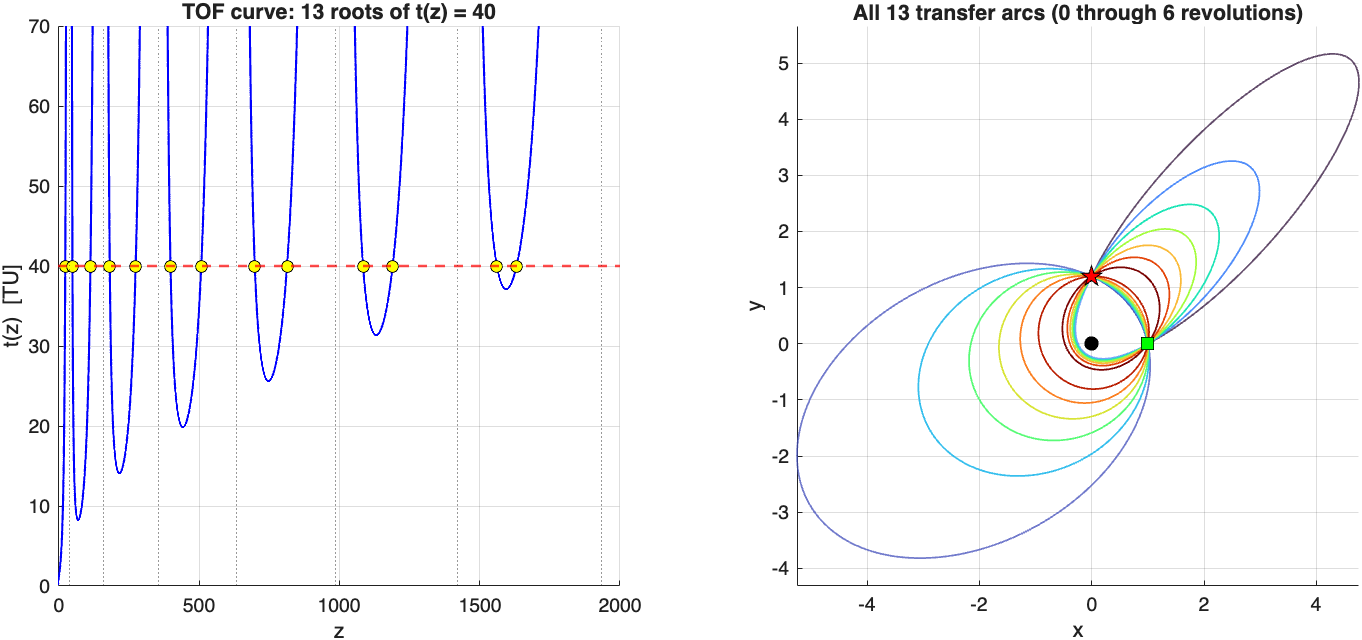
\includegraphics[width=0.98\textwidth]{expected_result.png}
\caption{The expected demo output. Left: the time-of-flight curve $t(z)$
with revolution-band boundaries (dotted), the $\Delta t = 40$ level (red),
and the 13 roots. Right: the 13 transfer orbits --- one 0-rev arc and six
left/right pairs --- all through $\rvec_1$ (green square) and $\rvec_2$
(red star).}
\label{fig:expected}
\end{figure}

% ==========================================================================
\section{What comes next}

\begin{enumerate}[leftmargin=*]
\item \textbf{Newton polish.} Replace pure bisection with
  bisection-safeguarded Newton using $dt/dz$ (Curtis Eq.~5.43 gives the
  closed form, including the $z = 0$ special value); watch iteration
  counts drop from $\sim$40 to $\sim$5. Then read how Izzo does it:
  \texttt{lambert\_original.cpp}'s \texttt{householder} iteration ---
  third-order convergence, 2--3 iterations --- on a \emph{bounded}
  variable $x$, which also eliminates the $\sinh$-overflow scan cap you
  met in Phase~C: the two formulations' trade-offs in one comparison.
\item \textbf{Porkchop plot.} Sweep departure and arrival dates for two
  given planet or satellite orbits (positions from an \emph{ephemeris} ---
  a table or model of where bodies are when), run your solver in the inner
  loop, and contour total $\Delta v$ --- the launch-window chart, and a
  solid stress test (thousands of calls, all geometries).
\item \textbf{Primer-vector hookup (P-OC6).} Along a two-impulse Lambert
  transfer, integrate $\ddot{\mathbf p} = G\mathbf p$ (your
  \texttt{orbit\_transfer} machinery) with Lawden's boundary conditions
  and evaluate $|\mathbf p(t)|$: does the arc satisfy the optimality
  conditions, or would a midcourse impulse lower the total $\Delta v$?
  This connects the two tutorials into one story.
\item \textbf{$\Delta v$-optimal wrapper.} A \texttt{minLambert}-style
  layer: scan $N$ and branch over your multi-rev output, add departure
  and arrival impulse magnitudes against given parking orbits, return the
  cheapest --- then compare architecture with pumpkyn's
  \texttt{minDeltaV}.
\item \textbf{CR3BP seeding.} Reproduce
  \texttt{pumpkyn.cr3bp.directLambert}'s pattern: your two-body solution
  as the initial guess, differentially corrected under three-body (CR3BP)
  dynamics via the state transition matrix --- the bridge from this
  tutorial to the cislunar/tulip-orbit work.
\end{enumerate}

\bigskip
\noindent\emph{Checkpoint provenance: all numbers from
\texttt{verify\_lambert\_checkpoints.m}, run headless on MATLAB R2025b on
2026-07-06. pyKep reference values from a standalone \texttt{clang++}
build of pumpkyn's bundled \texttt{lambert\_original.cpp} (the macOS MEX
toolchain is currently broken machine-wide); Vallado Example 7-5 anchors
the dimensional case. If you change the tutorial instance, re-run the
script and update the checkpoints.}

\end{document}
